% Simulation
\section{Simulation}
\subsection{General scheme}
\frame{To perform the simulation,
first we create a list of calls to attend,
with time between calls,
according to the exponential distribution
with parameter indicated by each demand point.

We define two types of events, 
calls and releases, 
each time a call is attended,
generates a release,
that is inserted in the list of events, 
indicating that a server is busy.
If all servers are busy, the call is sent to queue.
\begin{figure}
  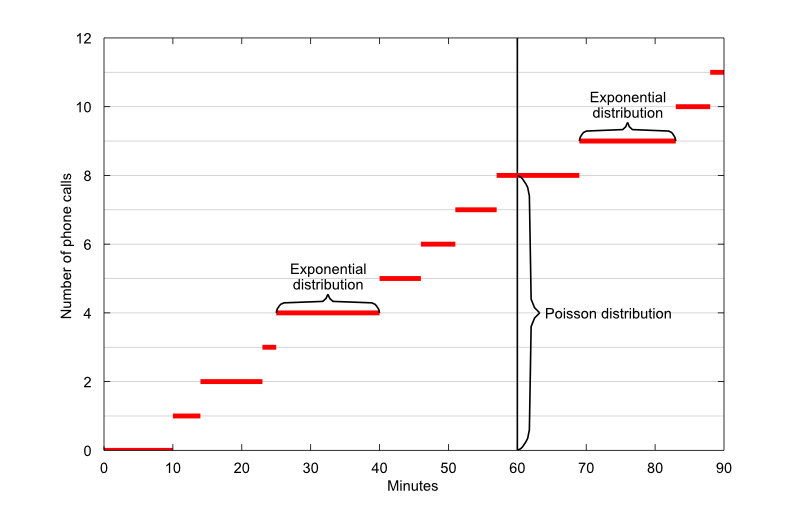
\includegraphics[width=7cm,keepaspectratio]{poisson_distribution}
\end{figure}
}
\frame{\begin{algorithm}
  \hline \vspace{3pt}
  \caption{Simulation}\label{alg_sim}
  \vspace{3pt} \hline
  \begin{algorithmic}[0]
    \Procedure{Simulation}{$demandpoints,Solution$}
    \State $Status.Solution \gets Solution$
    \State $Status.EventsList \gets GenerateCalls(demandpoints)$
    \State $Status.QueueList \gets EmptyList()$
    \State $Status.time \gets 0$
    \While{$Status.EventsList.notempty()$}
    \State $Event \gets EventsList.front()$
    \State $EventsList.remove.first()$
    \State $Event.process(Status)$
    \EndWhile
    \EndProcedure
  \end{algorithmic}
  \hline
\end{algorithm}
}

\begin{frame}
  \begin{algorithm}
    \hline \vspace{3pt}
    \caption{Process Call}\label{proc_call}
    \vspace{3pt} \hline
    \begin{algorithmic}[0]
      \Procedure{Call::process}{$Status$}
      \State $Status.time \gets call.time$
      \If{$IdleServerExist(Status)$}
      \State $server \gets NearestIdleServer(Status,call)$
      \State $Status.busy[server] \gets true$
      \State $release \gets Attend(call,server)$
      \State $Staus.EventList.InsertOrdered(release)$
      \Else
      \State $Status.QueueList.Insert(call)$
      \EndIf
      \EndProcedure
      \hline
    \end{algorithmic}
  \end{algorithm}
\end{frame}

\begin{frame}
  \begin{algorithm}
    \hline \vspace{3pt}
    \caption{Process Release}\label{proc_rel}
    \vspace{3pt} \hline
    \begin{algorithmic}[0]
      \Procedure{Release::process}{$Status$}
      \State $Status.busy[release.server] \gets false$
      \State $Status.time \gets release.time$
      \If{$Status.QueueList.notempty()$}
      \State $call \gets NearestCall(Status.QueueList,release.server)$
      \State $Status.busy[release.server] \gets true$
      \State $release \gets Attend(call,release.server)$
      \State $Staus.EventList.InsertOrdered(release)$
      \EndIf
      \EndProcedure
      \hline
    \end{algorithmic}
  \end{algorithm}
\end{frame}

\subsection{Results}
\begin{frame}
  The results obtained are:
  \begin{itemize}
  \item Attended Calls.
  \item Calls sent to the queue.
  \item Workloads.
  \item Service Time.
  \item Waiting Time.
  \item Travel Time.
  \item Arrival Time.
  \end{itemize}
\end{frame}

% redefine \VerbatimInput
\RecustomVerbatimCommand{\VerbatimInput}{VerbatimInput}%
{fontsize=\footnotesize,
 %
 frame=lines,  % top and bottom rule only
 framesep=2em, % separation between frame and text
 rulecolor=\color{Gray},
 %
 label=\fbox{\color{Black}Simulation.log},
 labelposition=topline,
 %
 commandchars=\|\(\), % escape character and argument delimiters for
                      % commands within the verbatim
 commentchar=*        % comment character
}

\begin{frame}
\VerbatimInput{Simulation.log}
\end{frame}

\subsection{Comparative}
\begin{frame}
  Some results obtained with the Simulation,
  can be compared with those obtained with the Jarvis approximation method. 
  \begin{itemize}
  \item Service Time.
  \item Workloads.
  \item Percentage of times that each server is assigned to each demand point.
  \end{itemize}
\end{frame}
